\documentclass[10pt,twocolumn]{article} 

\usepackage{oxycomps} % use the main oxycomps style file
\usepackage{amsmath}

\usepackage{array, booktabs, longtable}
\usepackage{graphicx}
\usepackage[x11names, table]{xcolor}
\usepackage{caption}
\DeclareCaptionFont{blue}{\color{LightSteelBlue3}}

\newcommand{\foo}{\color{LightSteelBlue3}\makebox[0pt]{\tiny\textbullet}\hskip-0.5pt\vrule width 1pt\hspace{\labelsep}}
\newcommand{\bfoo}{\raisebox{2.1ex}[0pt]{\makebox[\dimexpr2\tabcolsep]%
{\color{LightSteelBlue3}\tiny\textbullet}}}%
\newcommand{\tfoo}{\makebox[\dimexpr2\tabcolsep]%
{\color{LightSteelBlue3}$\boldsymbol \uparrow $}}%

\bibliography{references}

\pdfinfo{
    /Title (AI-Chinese Chess)
    /Author (Haotian wang)
}

\title{AI-Chinese Chess}

\author{Haotian wang}
\affiliation{Occidental College}
\email{hwang2@oxy.edu}

\begin{document}

\maketitle

\section{Problem Context}
    Xiangqi, also known as the elephant chess or the Chinese chess game, is a strategy board game for two players. It is one of the most popular board games in China. Chinese chess uses a square checkered board with 32 round pieces, 16 in each of the two colors red and black, placed and moving at intersections. The first player to "checkmate" the opponent's general wins. Just like any other chess or board games, Xianqi consist a great deal of combination moves and strategies. 
    People used to practice and play Xiangqi in the real world with either friends or arranged competitors in competitions. However, due to. the outbreak of Covid-19 pandemic, chess players often needs to be quarantined due to varies reasons, especially in China, where the lock down policies are extremely strict. Many of the competitions and practice arrangements are cancelled. Players are forced to either play online and practices online.  Players often have few options to choose who they can play to and where they can practice their skills. 
    
    AI and machine learn has been widely successful in applications for all kind of purposes in almost every field of work. In context, AI and machine learn has been solutions for various kind of strategy or decision making programs. AI is also used to test out human limits. The main advantage of using AI models to make decisions and plan strategies is that the the algorithms and computing power can provide the client the most accurate or best suited strategy with minimal bias factors in short time. Even though there are various kind of AI model for the Xiangqi already. However, the access for these projects are limited to very few player. Players are not able to access these AI models to train themselves. In addition, these models are generally made to test algorithms and compete with other AI models\cite{}. Since most AI models are used to test the limitations of the algorithms, the level of difficulty increases as well. General players who didn't reach that level will only defeat without knowing how to improve. 
    
\section{Technical Background}
	This implementation will require knowledge of reinforced deep learning, neural network, 
	Monte Carlo tree search, programming language and HTML. This implementation uses reinforcement learning based on deep neural network training. It adopts a self play learning model constructed by combining deep convolutional neural networks and Monte Carlo search tree algorithm, and uses MCTS algorithm to simulate chess moves that constantly change roles. 
	
	The deep convolutional neural network inputs mainly the current chessboard state and then outputs the likelihood of each move and the current player's victory rate via the deep convolutional neural network. If the deep convolutional neural network is \(f\), the deep neural network can be stated as follows:
	\[(p,v)=f_\theta(s)\]
	
	In addition,\(s\) represents the current state of the chessboard, \(p\) represents the likelihood of each move, and $p_a = Pr (a|s)$ represents the probability of each move. The current player's victory percentage is denoted by \(v\). The MCTS tree algorithm partially relies on the output results of \(f\) to direct MCTS to perform multiple simulation moves from the root node to the leaf node, so it can select a better winning rate strategy. Assume the MCST algorithm is \(\varphi_\theta\), then the MCST algorithm can be as follow:
	\[(\pi,z)=\varphi_\theta(p,v,N,Q)\]
	
	In this context, \(\pi\) represents the probability of each move output by the final reinforcement learning model, and \(z\) is the winning rate of the player who makes the first move in the game. The input of the MCST algorithm is the output \((p,v)\) of \(f_\theta\) combined with the number of visits \(N\) and the average action value \(Q\) in each iteration. When a game of chess is finished, the neural network's training goal is to maximize the similarity between $(p, v)$ and $(\pi, z)$, and then continually increase the neural network's processing power in self-learning.
	
	For each position the player moves, the algorithm use the latest deep neural network result to guide the MCTS to search for the move probability of each position. Each position consist \(I\) legal moves, then the move probability represents for the move corresponds to the probability of the move. The appropriate move is chosen for each position. Based on the above pattern, the until the game reaches the one player winning situation or check mate, the winner Z will be the next output. After the winner occurs, the neural network will be trained in the reverse direction according to the winner.
	
	\begin{figure}
        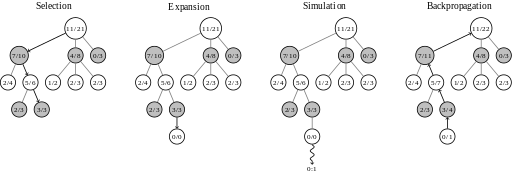
\includegraphics[width=\linewidth]{MCTS.png}
        \caption{MCTS}
        \label{fig1:Monte Carlo Tree search}
    \end{figure}
	
	Selection is the first stage in a Monte Carlo tree search. Begin with the root R and progress through the child nodes until you reach the leaf node L. The current game state is represented by the root, and a leaf is any node with a potential child but no simulation (play out) has yet been initiated. The section that follows goes into greater detail on a method of biasing the selection of child nodes that allows the game tree to expand towards the most promising moves, which is the essence of Monte Carlo tree search. Unless L finishes the game decisively (e.g., win/loss/draw) for either player, the second stage is expansion. Create one (or more) offspring nodes and select node C from one of them. Any legitimate move from the game position described by L is a child node. The third stage is simulation, which is accomplished by completing one random play out from node C. This process is also known as play out or roll out. A play out could be as easy as selecting uniform random moves till the game is over (for example in chess, the game is won, lost, or drawn). Back propagation is the final stage, which uses the results of the play out to update information in the nodes on the path from C to R.
	
	How to evaluate the strategy
	
\section{Prior Work}
    Artificial Inteligence and Machine learning algorithm models are one of the most widely employed methods for decision and strategy projects. In this section we will focus on the prior works done in using AI and ML models implemented in other strategy games, especially the Monte Carlo tree search implementation, as it is the one of the most important part of this project 
\subsection{Alpha Go Zero}
    The game "Go" is played with a rectangular board and black and white circular pieces. There are 19 lines and 361 intersections on the regular board, and the pieces must move on the intersections where spaces are not forbidden. Because Black has a first move advantage, Black is artificially required to give White an eye at the end of the game. AlphaGo Zero is a computer software that combines a deep neural network with an advanced search tree. As an input, these neural networks process a description of the Go board through a number of network layers comprising millions of neuron-like connections. The "policy network," a neural network, chooses the next move to play. The "value network," the other neural network, predicts the game's winner. We exposed AlphaGo Zero to a variety of amateur games in order to help it build a grasp of reasonable human play. Then we let it play thousands of times against different versions of itself, each time learning from its mistakes. AlphaGo Zero evolved over time, becoming ever stronger and better at learning and decision-making. This is referred to as reinforcement learning. AlphaGo Zero went on to defeat Go world champions in many worldwide arenas, establishing himself as the greatest Go player of all time.In a Go game, AlphaGo Zero builds a local policy to sample the next move using MC Tree Search. MCTS looks for potential moves and stores the results in a search tree. As more searches are made, the tree and its information grow in size. 
    
    

\subsection{Deep blue}
    Deep Blue was a chess-playing expert system that ran on a one-of-a-kind IBM supercomputer. It was the first computer to win a game and the first to win a match against a defending world champion in regular time.
    Deep Blue's evaluation function was first developed in a generalized manner, with many parameters still to be defined. Thousands of master games were analyzed to get the values for these factors. The evaluation function was then divided into 8,000 pieces, many of which were intended for specific roles. The opening book featured almost 4,000 positions and 700,000 grand master games, while the endgame database included many six-piece endgames as well as all five and fewer piece endgames. An supplementary database known as the "extended book" summarizes whole grand master games. To identify opening moves, the algorithm combines its ability to search 200 million chess positions per second with summary information from the extended book.
    \begin{figure}
        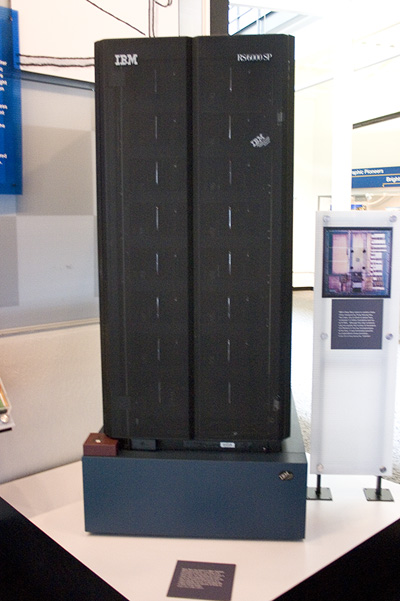
\includegraphics[width=90]{Deep_Blue.jpg}
        \caption{Deep Blue cabinets}
        \label{fig2:Deep Blue}
    \end{figure}
    
\section{Methodology}
    For this AI-Chinese chess project, i propose to Machine learning, specifically Reinforcment learning and the Monte Carlo Tree search algorithm. In addition, This project will be hosted online using HTML.
    
\subsection{Language}
\subsection{obtain Data}
\subsection{Pre-process Data}
\subsection{Input data}
\subsection{Built-in GUI}
\subsection{Self-Play}
\subsection{Training}
\subsection{Evaluator}
\subsection{Supervised Learning}
\subsection{Website }
\section{Evaluation}
    To Evaluate the success of this project, i plan to to evaluate it using the following three methods: invitation to XiangQi players to compete with the model and provide feed back. Feed the model data from after training period and compare the outputted winning rate against other published AI-chinses chess models to see if the way i train the model succeeded or not. Post the game with the model on a website and invite people around the world to test the training function, if the feed back came back positive, then that means the training purpose is achieved. 
    Based on the players feed back, we can optimize the model in the following feedback to best assist players to train and challenge themselves. 
\begin{itemize}
    \item is the level of difficulty to hard or too easy for the player; 
    \item is the model performing without mistakes;
\end{itemize}
    
\section{Ethical Consideration}

\section{Limitations, Future Work, and Conclusion}

\section{Proposed Timeline}

\renewcommand\arraystretch{1.4}\arrayrulecolor{LightSteelBlue3}
\captionsetup{font=blue, labelfont=sc, labelsep=quad}
\begin{longtable}{@{\,}r <{\hskip 2pt} !{\foo} >{\raggedright\arraybackslash}p{5cm}}
 \caption{Timeline} \\[-1.5ex]
\toprule
\addlinespace[1.5ex] 
 \multicolumn{1}{c!{\tfoo}}{}& \\[-2.3ex]
May - August & Collect real player moves data; Pre-process data into data sets for data analysis\\
September & establish the coding and data prepare for training or begin training\\
October & Train Model\\
November & Post online to more training and testing for feedback\\
December & Finish COMPs paper and present findings\\
 \multicolumn{1}{c!{\bfoo}}{}&
\end{longtable}

\printbibliography 

\end{document}